%%% ELS includes
% * <sfujimori112256@gmail.com> 2017-05-23T14:15:19.404Z:
% 
% comment from SF
% 
% ^ <sfujimori112256@gmail.com> 2017-05-24T18:49:42.852Z.
\documentclass[review]{elsarticle}
\usepackage{lineno,hyperref}
\modulolinenumbers[5]
\journal{Environmental Modelling \& Software}
\bibliographystyle{elsarticle-num}
%%%

%%% General usepackages, definitions, etc.
%%%%% Packages and related options
%%
%% Note, order matters!
%%
\usepackage[acronym,toc]{glossaries}
\usepackage{graphicx}
\usepackage{booktabs} % nice rules for tables
\usepackage{microtype} % if using PDF
\usepackage{hyperref}
\usepackage{amsmath}
\usepackage{moreverb} % for verbatim snippets of code
\usepackage{fancyvrb}
\usepackage{tabularx} % for tables with line breaks
\usepackage{threeparttable} % for tables with notes
\usepackage[capitalize, noabbrev]{cleveref} % for reference multiple figures
\usepackage{calc} % allows for arithmetic on latex variables
\usepackage{float} % allows for figures to be placed explicitly
\usepackage{algorithm2e} % for algorithms
\usepackage{subfig}
\usepackage{multirow} % combining rows in tables
\usepackage{footnote}
\usepackage{titlesec} % for using \titleformat
\usepackage{bashful}
\usepackage{xspace}
\usepackage{color}
\definecolor{listinggray}{gray}{0.9}
\definecolor{lbcolor}{rgb}{0.9,0.9,0.9}
\lstset{
    %backgroundcolor=\color{lbcolor},
    language={C++},
    tabsize=4,
    rulecolor=\color{black},
    upquote=true,
    aboveskip={1.5\baselineskip},
    belowskip={1.5\baselineskip},
    columns=fixed,
    extendedchars=true,
    breaklines=true,
    prebreak=\raisebox{0ex}[0ex][0ex]{\ensuremath{\hookleftarrow}},
    frame=single,
    showtabs=false,
    showspaces=false,
    showstringspaces=false,
    basicstyle=\scriptsize\ttfamily\color{black},
    keywordstyle=\color[rgb]{0,0,1.0},
    commentstyle=\color[rgb]{0.133,0.545,0.133},
    stringstyle=\color[rgb]{0.627,0.126,0.941},
    numberstyle=\color[rgb]{0,1,0},
    identifierstyle=\color{black},
    captionpos=t,
}
\lstdefinestyle{BashOutputStyle}{
  basicstyle=\small\ttfamily,
  numbers=none,
  frame=tblr,
  columns=fullflexible,
  backgroundcolor=\color{blue!10},
  linewidth=0.9\linewidth,
  xleftmargin=0.1\linewidth
}
%%%%% 

%%%%% Helpers

\newcommand{\code}[1]{\lstinline[basicstyle=\ttfamily\color{black}]|#1|}
\newcommand{\codeb}[1]{\texttt{#1}}
\newcommand{\units}[1] {\:\text{#1}}%
\newcommand{\TODO}[1]{\textbf{TODO: #1}}

%%% gases
\newcommand{\cotwo}{CO\textsubscript{2}~}
\newcommand{\nox}{NO\textsubscript{x}}
\newcommand{\noxx}{NO\textsubscript{x}~}
\newcommand{\nht}{NH\textsubscript{3}}
\newcommand{\nhtt}{NH\textsubscript{3}~}

%%% units
\newcommand{\wm}{$\frac{\text{W}}{\text{m}^2}$}

%%% detect beginning of sentences and capitalize appropriately
\sfcode`\.=1001
\sfcode`\?=1001
\sfcode`\!=1001
\sfcode`\:=1001
\newcommand\secref[1]{\ifnum\spacefactor=1001 Section \ref{#1}\else section \ref{#1}\fi}
% this seems like a limitation of sfcode (an error occurs if at the beginnig of
% a paragraph) Accordingly, this can be used manually as
% needed. http://comments.gmane.org/gmane.comp.tex.texhax/17631
\newcommand\Secref[1]{ Section \ref{#1}}
%%%

\makeatletter
\newcommand\footnoteref[1]{\protected@xdef\@thefnmark{\ref{#1}}\@footnotemark}
\makeatother


%%% General setup
\graphicspath{{./figs/}}
%\include{acros}
\makeglossaries

\begin{document}

%%% ELS input
\begin{frontmatter}

\title{A Methodology and Implementation of Automated Emissions Harmonization for Use in Integrated Assessment Models}

%% Group authors per affiliation:
\author[iiasa]{Matthew J. Gidden\corref{corref}}
\ead{gidden@iiasa.ac.at}
\cortext[corref]{Corresponding author}

\author[iiasa,nies]{Shinichiro Fujimori}
\author[iiasa]{Keywan Riahi}

\address[iiasa]{International Institute for Applied Systems Analysis,
  Schlossplatz 1, A-2361 Laxenburg, Austria}
\address[nies]{National Institute for Environmental Studies, Tsukuba, Japan}

\begin{abstract}
Harmonization describes the process of calibrating Integrated Assessment Model
(IAM) GHG and air pollutants results with a new source of historical emissions trajectories. To date,
harmonization has been performed separately by individual modeling teams through
% * <sfujimori112256@gmail.com> 2017-05-24T19:26:26.142Z:
% 
% > harmonization has been performed separately by individual modeling teams 
% I think harmonization is not done. We just report the direct model outputs.
% 
% One of the ways to  make the background is that earlier IPCC scenarios (SRES and RCPs) did not document the harmonization method and far from transparent.
% 
% ^.
the use of expert opinion and solicitation. As models and their results become
more complex in both regional and sectoral dimensions, an automated approach to
choosing harmonization methods becomes necessary. This work describes a novel
% * <sfujimori112256@gmail.com> 2017-05-24T20:13:08.493Z:
% 
% > novel
% It would be better to stress how novel and useful.
% 
% ^.
methodology for determining such harmonization methods and an open-source Python
code base for implementing the methodology. Results are shown for two example
scenarios using the MESSAGE-GLOBIOM IAM that satisfactorily harmonize over 98\%
of the total emissions trajectories.
\end{abstract}

\begin{keyword}
Integrated Assessment Modeling, Harmonization, Climate Change, Air Pollution 
\end{keyword}

\end{frontmatter}

\linenumbers 
%%%

\newpage

\section{Introduction}

Integrated Assessment Models (IAMs) are tools used to understand the complex
interactions between energy systems, economic systems, land use, the climate,
and air pollution. IAMs provide global projections of
systemic change by dividing the world into a number of representative regions
(typically 10 to 30), the definition of which is distinct for each model
\cite{krey_global_2014}. Results from IAMs are integral in a number of
international studies, which notably include projections of climate and economic
futures. Recently, the IAM community has developed scenarios based on the Shared
% * <ssmith@pnnl.gov> 2017-07-01T03:11:26.621Z:
% 
% > flagship
% Suggest different word. "comprehensive" is one possibility.
% 
% ^ <ssmith@pnnl.gov> 2017-07-01T03:11:57.571Z.
Socioeconomic Pathways (SSPs) \cite{van_vuuren_energy_2017, fricko_marker_2017,
  fujimori_ssp3:_2017, calvin_ssp4:_2017, kriegler_fossil-fueled_2017} which
quantify a variety of potential global futures. The SSPs are  designed
to be used in  research that include earth system
model (ESM) simulations, climate impact, adaptation and climate mitigation
studies. 

While IAMs are implemented in myriad ways, including simulation and
optimization, the core inputs and outputs  are similar across different
models. Modeling teams incorporate  data on energy systems, land
use, economics, demographics and emissions sources and concentrations, among other
data, in order to provide consistent existing trajectories of modeled
variables. The models then provide estimates of future trajectories of these
variables under various socioeconomic and technological assumptions as well as
proposed policy constraints, e.g., targets for future Greenhouse Gas (GHG)
emissions.

The emissions trajectories calculated by IAMs are critical inputs for ongoing,
worldwide scientific community efforts in the Coupled Model Intercomparison
Project Phase 6 (CMIP6) \cite{eyring_overview_2016}, which is utilizing a number
of marker SSP scenarios developed by the IAM community
\cite{oneill_scenario_2016}. These trajectories are endogenously calculated by
modeling the individual technologies and sectors that contribute towards the
emissions of different air pollutants and GHGs as well as various mitigation
technologies. However, the historical emissions starting points of  models can differ by
large amounts depending on the region, sector, and emissions species.

In practice, IAMs calculate the total source intensity of emitting technologies,
for example the total activity of coal power plants in China, and incorporate
emissions-intensity factors for individual gas species, for example the quantity
of sulfur emissions from coal plants per megawatt-hour of production. Models are generally \textit{calibrated} to historical data sources in one or more base years. Due to the sometimes large uncertainties
in historical datasets, results in the historical period may differ between
models. Models also differ in their choice of base-year, which may lag behind available inventory data. In addition, models have varying sectoral, regional, and fuel aggregations.

The
global climate change community has recently developed a new global historical
emissions dataset for both anthropogenic  emissions (i.e., the Community
Emissions Data System (CEDS) \cite{hoesly_historical_2017} and open-burning land-use and land-use change (LULUC)
emissions \cite{van_marle_historic_2017}) which, in
% * <sfujimori112256@gmail.com> 2017-06-07T09:59:35.820Z:
% 
% > land-use change (LUC) emissions \cite{van_marle_historic_2017}
% I think this one also anthropogenic
% 
% ^ <maarten.vandenberg@pbl.nl> 2017-07-03T20:46:42.206Z:
% 
% I think so too, however I believe the GFED also contains natural emissions.
%
% ^.
conjunction with the SSP IAM trajectories, will be used for climate-related
modeling exercises of CMIP6.

When participating in intercomparison exercises in which a consistent historical starting point is required (e.g., in CMIP6), model teams incorporate a
single, common historical dataset through \textit{harmonization}. Harmonization describes the process of
adjusting model results to match the selected historical time series  such that the resulting future trajectories are also consistent with the
original modeled results. In the emissions context, this means that each
individual combination of model region, model sector, and emissions species must
be harmonized. Depending on the total number of model regions, sectors, and
emissions species, this can require the selection of thousands to
tens-of-thousands of harmonization methods.

Harmonization has been addressed in previous studies as it is a common practice
in the IAM and climate change communities. For example,
\cite{meinshausen_rcp_2011} describes the use of scaling routines for the 5
regions used in the Special Report on Emissions Scenarios (SRES)
\cite{nakicenovic2000}; however, only total emissions were harmonized in the
exercise, thus there is no sectoral dimension. Further,
\cite{rogelj_discrepancies_2011} describes the impacts of choosing various
harmonization routines on future trajectories. During the evaluation of the
Representative Concentration Pathways (RCPs), IAM results have been harmonized
by sector and the 5 RCP global regions
\cite{vuuren_representative_2011}. Importantly, the choice of harmonization
method to date has been determined via expert solicitation and has generally
been applied to all trajectories for a given class of emissions species.

Climate modeling efforts have continued to progress, demanding increased spatial
and sectoral resolution from IAMs. Furthermore, a new generation of climate
scenarios which combines aspects of both the RCPs and SSPs have been developed
in order to incorporate both physical and socioeconomic detail. In order to
address the growing dimensionality of model outputs and support ongoing scenario
generation and analysis efforts while still providing a consistent and
scientifically rigorous harmonization procedure, an automated process for
determining harmonization methods is needed. The use of an automated,
documented, and openly available harmonization mechanism additionally allows for
full procedural reproducibility and for direct participation by additional
modeling teams not involved in the original exercise.

The remainder of this paper describes the methodology and implementation of the
harmonization code base \code{aneris} \cite{matthew_gidden_2017_802832}, written in the Python
% * <maarten.vandenberg@pbl.nl> 2017-07-03T21:12:05.654Z:
% 
% > the
% > \code{aneris} code base \cite{matthew_gidden_2017_802832
% perhaps something like: "the harmonization code base \code{aneris}", to be explicit.
% 
% ^.
programming language (detailed documentation available
\href{http://mattgidden.com/aneris/}{online}). Section \ref{sec:meths} provides
a detailed description of the underlying mathematical components of
\code{aneris} as well as the code workflow. The results of applying the
automated harmonization mechanism on two example IAM scenarios, one with
emissions growth and another with emissions mitigation, is presented in Section
\ref{sec:results}. Finally, the general effectiveness and potential future
improvements on the automated methodology is discussed in Section
\ref{sec:future}.

\section{Methodology \& Implementation}\label{sec:meths}

\subsection{Harmonization Methods}

IAM emission results are provided along temporal (normally half decade or
decade), spatial (i.e., model regions), gas species, and sectoral
dimensions. Each individual temporal trajectory, i.e., unique combinations of
regions ($r$), species ($g$), and sectors ($s$), must be harmonized to the
initial modeling period. Given a model trajectory, $m_{r, g, s}(t)$, historical
values, $h_{r, g, s}(t)$, and model base year, $t_i$, a harmonized trajectory
needs to be calculated. The \textit{harmonization quality} of a trajectory,
i.e., how well a given harmonization algorithm performs, depends on a number of
factors. Of chief import is the faithful representation of the original,
unharmonized, trajectory as well as the representation of negative trajectories
(i.e., if a trajectory becomes negative, both the timing and total magnitude
should be as close as possible) which are of critical importance for cumulative
\cotwo calculations.

In previous studies \cite{meinshausen_rcp_2011,rogelj_discrepancies_2011}, two
\textit{families} of methods have been used: those that operate on the ratio of
base year values (i.e., $\frac{h(t_i)}{m(t_i)}$) and those that operate on the
offset of base year values (i.e., $h(t_i) - m(t_i)$). A number of the classic
methods are implemented in \code{aneris} including ratio-convergence shown in
Equation \ref{eqs:ratio}, offset-convergence shown in Equation \ref{eqs:offset},
and interpolation shown in Equation \ref{eqs:interpolate}. The convergence
factor, $\beta$, scales linearly from 1 to 0 over $[t_i, t_f)$ and is shown in
  Equation \ref{eqs:factor}. In all equations the region, species, and sector
  indices have been dropped for clarity. Each equation is a function of time,
  model trajectory, historical trajectory, base year ($t_i$), and a convergence
  year ($t_f$), at which point the harmonized trajectory converges to the
  unharmonized trajectory. \codeb{aneris} provides a number of methods to choose
  from for each of the harmonization families. A summary of all available
  methods is provided in Table \ref{tab:meths}.


\begin{equation}\label{eqs:factor}
  \beta(t, t_i, t_f) =
  \begin{cases}
    1 - \frac{t - t_i}{t_f - t_i},& \text{if } t < t_f\\
    0,                        & \text{otherwise}
  \end{cases}
\end{equation}

\begin{equation}\label{eqs:ratio}
  m^{rat}(t, m, h, t_i, t_f) = [\beta(t, t_i, t_f) (\frac{h(t_i)}{m(t_i)} - 1) + 1] m(t)
\end{equation}

\begin{equation}\label{eqs:offset}
  m^{off}(t, m, h, t_i, t_f) = \beta(t, t_i, t_f) (h(t_i) - m(t_i)) + m(t)
\end{equation}
  
\begin{equation}\label{eqs:interpolate}
  m^{int}(t, m, h, t_i, t_f) =
  \begin{cases}
    \beta(t, t_i, t_f) (h(t_i) - m(t_f)) + m(t_f), & \text{if } t < t_f\\
    m(t), & \text{otherwise}
  \end{cases}
\end{equation}


\begin{table}[h!]
\centering
\caption{All Harmonization Methods Provided in \code{aneris}}
\label{tab:meths}
\begin{tabular}{|l|l|l|}
\hline
Method Name                             & Harmonization Family & Convergence Year\\
\hline
\code{constant\_ratio}                  & ratio              & $t_f = \infty$\\
\code{reduce\_ratio\_<year>}            & ratio              & $t_f = $\code{<year>}\\
\code{constant\_offset}                 & offset             & $t_f = \infty$\\
\code{reduce\_offset\_<year>}           & offset             & $t_f = $\code{<year>}\\
\code{linear\_interpolate\_<year>}      & interpolation      & $t_f = $\code{<year>}\\
\hline
\end{tabular}
\end{table}

\subsection{Default Method Decision Tree}\label{sec:tree}

A \textit{decision tree} approach has been implemented in \codeb{aneris} which
provides a systematic and documented decision-making process to determine the
preferred harmonization algorithm. In order to provide reasonable
\textit{default} methods, the historical trajectory, unharmonized model
trajectory, and relative difference between history and model values in the
harmonization year are analyzed. The decision tree used in this analysis is a
result of collaborative efforts between IAM teams and is shown graphically in
Figure \ref{fig:decision_tree}.


\begin{figure}
  \begin{center}
    \includegraphics[width=\textwidth]{decision_tree.pdf}
    \caption[]{
      \label{fig:decision_tree}
      The default method decision tree used in the \code{aneris} software
      library. For all decisions, upper (purple) branches represent a ``yes''
      response and lower (orange) branches represent a ``no'' response. The
      coefficient of variation, $c_v$, is defined in Equation \ref{eqs:cov},
      $dH$ is defined as $\left|\frac{h(t_i) - m(t_i)}{h(t_i)}\right|$, and
      decision-making thresholds for $c_v$ and $dH$ are described below. Methods
      labeled in \textit{green} are likely to closely match unharmonized
      results, methods in \textit{yellow} will likely somewhat match
      unharmonized results, and methods in \textit{red} can be expected to have
      a large relative difference between harmonized and unharmonized results.}
  \end{center}
\end{figure}

A number of characteristics impact the decision of which default method to
select based on the effect of the characteristic on the potential harmonized
trajectory. For example, it is possible for models to report zero values in the
harmonization year in situations in which technologies are introduced in future
time periods in regions or for sectors which produce an emissions species that
is absent in the initial modeling period. In such cases, an offset method is
required as a ratio method would mask future emissions and erroneously harmonize
the trajectory. 

In most cases, however, models do report values in the harmonization
year. Figure \ref{fig:cases} displays a number of example trajectories which
highlight the possible issues resulting from harmonizing model results in
different contexts. When model and historical values are relatively close, a
convergence method is chosen in order to be as representative as possible to the
underlying unharmonized model results (Figure \ref{fig:cases}, Panel
\code{a}). If values are not close, the constant ratio method is chosen in order
to provide reasonable trajectories that still incorporate modeled effects
(Figure \ref{fig:cases}, Panel \code{b}). 

Models can additionally report negative emissions in certain contexts which must
be taken into account during harmonization. Such a case is possible for gas
species which can be extracted from the environment and stored, as is the case
for \cotwo in future scenarios with climate mitigation. If a model provides a
trajectory that transitions from positive to negative emissions and base year
results are similar, then a convergence method is used in order to guarantee
capture of this transition in a representative fashion (Figure \ref{fig:cases},
Panel \code{c}). If the discrepancy in base year results is large, it is
possible for a negative trajectory to be inappropriately harmonized to a
positive, but decreasing, trajectory. As such, the constant ratio method is
chosen (Figure \ref{fig:cases}, Panel \code{d}).

\begin{figure}
  \begin{center}
    \includegraphics[width=\textwidth]{cases.pdf}
    \caption[]{
      \label{fig:cases}
      The effect of different harmonization routines on model trajectories under
      ``normal'' circumstances (Panel \code{a}), when there is a large
      difference between historical and model values in the harmonization year
      (Panels \code{b} and \code{d}), and when model trajectories result in
      negative emissions by the end of the modeling time horizon (Panels
      \code{c} and \code{d}). Identical model trajectories are used in each row
      (Panels \code{a}, \code{b}; \code{c}, \code{d}). In each column,
      historical values are increased in the base year by an order of magnitude
      (from 10 to 100). In each Panel, a subset of the potential routines
      provide a better harmonization quality than others as described in the
      text.
    }
  \end{center}
\end{figure}

Temporal variability of the historical trajectory is also an important
characteristic when considering the choice of harmonization method.  Emissions
from forest and grassland fires, for example, vary from year to year due to a
combination of meteorological conditions and anthropogenic drivers. Land use
emissions in many IAMs are modeled using average emission factors and do not
capture conditions in a specific year. A longer convergence horizon is thus
desired in order to incorporate highly variable historical data with modeled
results as is consistency in harmonization method because the effects are
modeled similarly across regions and species. In order to detect emissions with
a high amount of variation, a measure of the coefficient of variation, $c_v$, of
the first derivative of the historical trajectory is calculated using the
standard deviation, $\sigma$, and the mean, $\mu$, as shown in Equation
\ref{eqs:cov}.

The value of $c_v$ is then tested against a threshold, $\tau_{c_v}$. To
determine this threshold, an analysis of the recent CEDS and LUC historical data
has been performed. Figure \ref{fig:cov} shows the distribution of LUC $c_v$s
and non-LUC $c_v$s as determined for historical data aggregated to the model
regions of 5 different IAMs involved in the SSP process. A threshold value of
$\tau_{c_v} = 20$ has been chosen based on these observations as it
optimally divides the two distributions. Importantly, tails of the LUC and
non-LUC overlap, thus there are both false positives (~7\% of non-LUC
trajectories) and false negatives (~10\% of LUC trajectories). However, as any
regional definition is model dependent and thus any regional aggregation is
possible an automated detection mechanism is necessary.

\begin{equation}\label{eqs:cov}
    c_v =  \frac{\sigma(h^{\prime}(t))}{\mu(h^{\prime}(t))}
\end{equation}


\begin{figure}
  \begin{center}
    \includegraphics[width=\textwidth]{cov.pdf}
    \caption[]{
      \label{fig:cov}
      The distribution of $c_v$ values for LUC and non-LUC historical
      trajectories is shown. CEDS historical data \cite{hoesly_historical_2017}
      is used for non-LUC data and \cite{van_marle_historic_2017} is used for
      LUC data. All historical data has been aggregated from countries to IAM
      model regional definitions, and all gas species included in the historical
      data sets are included in the analysis. The solid black line indicates the
      threshold value, $\tau_{c_v}$, used by default in \code{aneris}.  }
  \end{center}
\end{figure}

Finally, consideration is taken with respect to the relative difference between
the historic and model values in the harmonization time period. In order to
investigate the possible values that these relative differences can take, the
IAM values used in the SSP and (ongoing) CMIP6 inter-comparison
exercises are used. A distribution of these differences for all models in the
study is presented in Figure \ref{fig:dh}. Given the available data, a threshold
value of $\tau_{dH} = 50$\% was chosen to be used as a default in \code{aneris}.

\begin{figure}
  \begin{center}
    \includegraphics[width=\textwidth]{dh.pdf}
    \caption[]{
      \label{fig:dh}
      The distribution of relative differences between model and historical
      values in the harmonization year is shown. The solid black line indicates
      the 50\% threshold value, $\tau_{dH}$, used by default in \code{aneris}.
    }
  \end{center}
\end{figure}

\subsection{\code{aneris} Workflow}\label{sec:workflow}

The full \code{aneris} workflow is comprised of a number of components shown
graphically in Figure \ref{fig:workflow}. Unharmonized model data and a
run-control configuration are read in via an Excel spreadsheet. Data is assumed
to be in the IAMC format, i.e., using \code{Model}, \code{Scenario},
\code{Region}, \code{Variable}, and \code{Unit} columns in addition to columns
representing each modeled time period.

Users are able to control the harmonization process via a number of options. The
primary mechanism by which users control the process is by providing
\textit{override} methods for any combination of region and variable (i.e.,
sector and gas species).  In practice, it may be possible that not all default
methods chosen will provide robust harmonized trajectories, especially if there
is a significant difference between historical and model values in the
harmonization year, if there is significant upward or downward movement in the
model trajectory, or if there are known discrepancies in sectoral definition
between the IAM and historical data source. In such cases, override methods can
ameliorate the issues associated with the default method choice. In order to
help identify these cases, harmonization \textit{diagnostics} are provided which
analyze the relative difference between harmonized and unharmonized trajectories
at their mid (if $> 400$\%) and end-points (if $> 200$\%). If override methods
are provided, they are used instead of the default methods as determined by the
default method decision tree. Furthermore, users can set the above-mentioned
thresholds as well as the LUC method used in the decision tree (see Figure
\ref{fig:decision_tree}). Further detail of input parameters can be found
\href{http://mattgidden.com/aneris/config.html}{online}.

\begin{figure}
  \begin{center}
    \includegraphics[height=0.9\textheight]{aneris-workflow.pdf}
    \caption[]{
      \label{fig:workflow}
      The full harmonization process as executed by \code{aneris}. Operations
      that can be configured with user-based input configurations are shown in
      purple. The core harmonization process is shown in yellow.  }
  \end{center}
\end{figure}

Input data then undergoes a cleaning operation, which adds (null) model
trajectories that exist in the historical data set but are not provided by the
model input and detects any issues that would cause the harmonization process to
fail. The methods used to harmonize the data are then determined and the
harmonization process is executed. Upon completion of the harmonization process,
aggregation of common analysis regions is performed. A common regional
aggregation used in the IAM community was defined in the Representative
Concentration Pathways (RCPs) \cite{vuuren_representative_2011}, shown in Figure
\ref{fig:regions}. Finally, any exogenous trajectories the user provides are
added. Exogenous trajectories are normally provided for unmodeled gases with
well-accepted scenario trajectories, e.g., chlorofluorocarbons provided by WMO
\cite{wmo2014}. Upon completion, the harmonized trajectories and meta data
regarding the harmonization process are returned. A description of all returned
meta data is provided in Table \ref{tab:metadata}.


\begin{figure}
  \begin{center}
    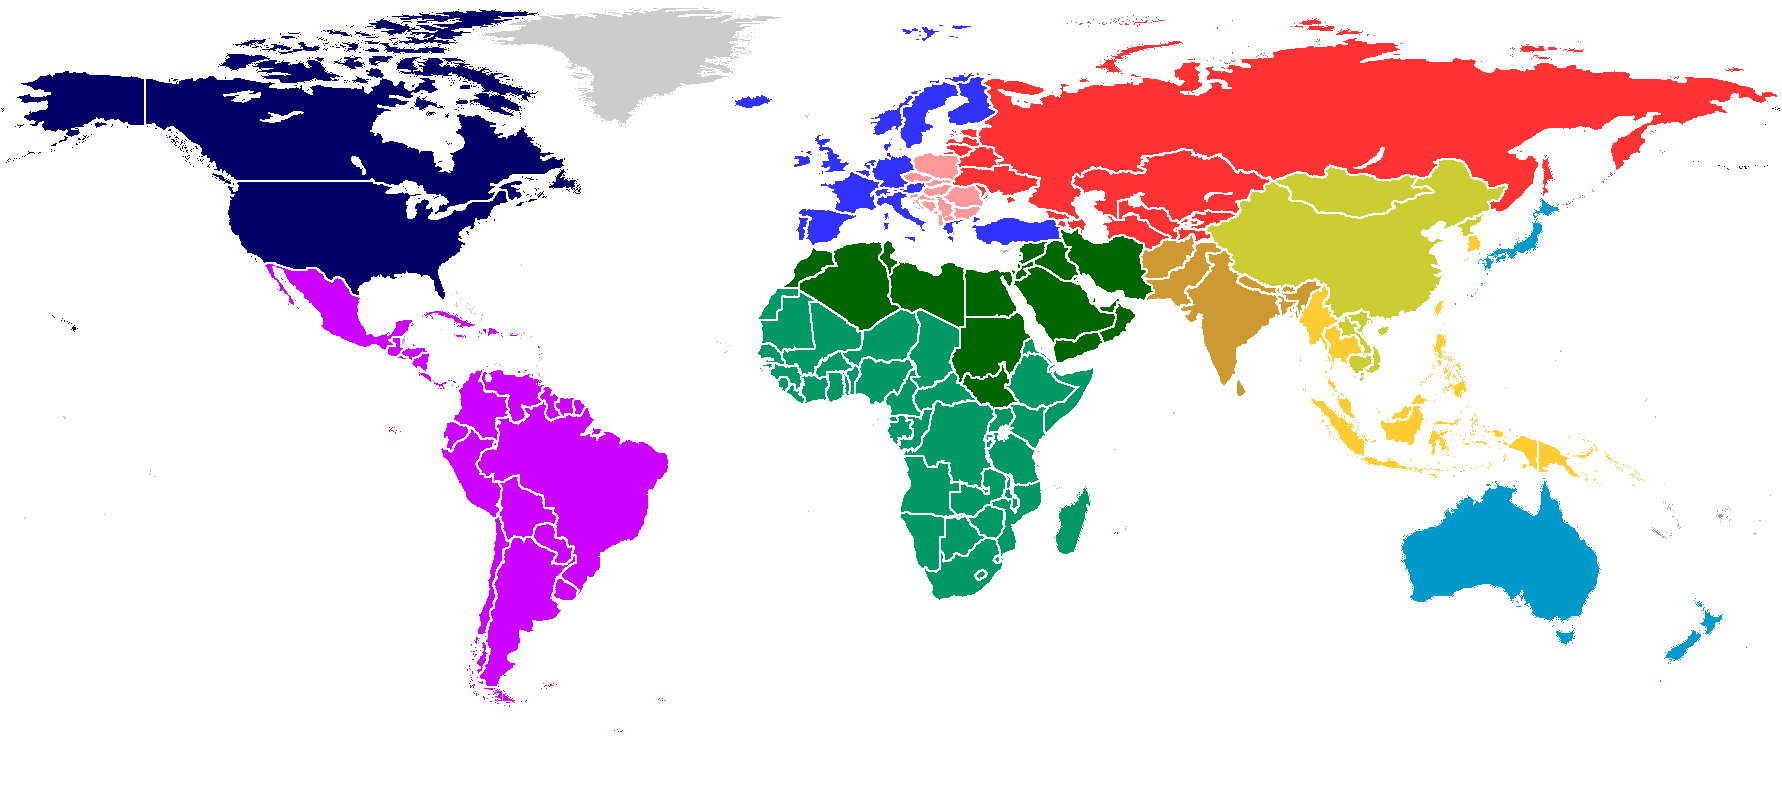
\includegraphics[width=\textwidth]{MESSAGE_11-5regions_map.pdf}
    \caption[]{
      \label{fig:regions}
      The 5 regions used in the RCPs with their 11-region constituents: Asia
      (Central Asia, South Asia, Pacific Asia) [yellows], Latin America
      [magenta], the Middle East and Africa [greens], the OECD (North America,
      Western Europe, and Pacific OECD) [blues], and the Reforming Economies
      (Eastern Europe and Former Soviet Union) [reds].  }
  \end{center}
\end{figure}


\begin{table}[]
\centering
\caption{Meta data provided by the \code{aneris} harmonization routine. This meta data is provided for every combination of region, sector, and emissions species.}
\label{tab:metadata}
\begin{tabular}{|p{2cm}|p{8cm}|}
\hline
\textbf{Column}       & \textbf{Description}                                      \\
\hline
\hline
method       & The harmonization method used.                                               \\
\hline
default      & The default harmonization method as determined by the default decision tree. \\
\hline
override     & The method provided as an override (if any).                                 \\
\hline
offset       & The offset value between history and model in the harmonization year.        \\
\hline
ratio        & The ratio value between history and model in the harmonization year.         \\
\hline
cov          & The coefficient of variation value of the historical trajectory.                           \\
\hline
unharmonized & The unharmonized value in the harmonization year.                            \\
\hline
history      & The historical value in the harmonization year.                             \\
\hline
harmonized   & The resulting harmonized value in the harmonization year.\\
\hline
\end{tabular}
\end{table}

\section{Results \& Conclusions}

\subsection{A Harmonization Test Case}

In order to test the \code{aneris} harmonization procedure, results from the IAM
MESSAGE-GLOBIOM \TODO{CITE} was processed. Two scenarios from the Shared Socioeconomic
Pathways scenario library \TODO{CITE} are investigated. The reference SSP2, or
``middle of the road'' is chosen first because MESSAGE-GLOBIOM is the marker
scenario for this SSP. Notably, emissions from multiple sectors tend to increase
in SSP2, thus testing the harmonization mechanism with a increasing emission
pathway. Additionally, the SSP-45 scenario is chosen, where the ``45''
designation refers to a scenario with end-of-century emissions resulting in
approximately a 4.5 $\frac{\text{W}}{\text{m}^2}$ warming effect by the end of
the century, due to both warming from Greenhouse Gases (GHGs) and fluoridated
gases as well as cooling from aerosols. In this scenario, mitigation
technologies and policies are enacted causing a general reduction in pollutants
and GHGs, including (eventual) negative CO2 emissions in some regions and
sectors due to carbon capture and sequestration and afforestation. This scenario
explores the harmonization mechanism's response to generally decreasing emission
trajectories.

MESSAGE-GLOBIOM includes a representation of 11 distinct regions which can be
mapped directly to the 5-region definition used in the RCPs. Historical data is
taken from CEDS and LUC \TODO{get correct name}, which comprise 10 separate
pollutant and GHG species and 13 sectors. Therefore, a total of 1430 distinct
trajectories were harmonized.

The effect of harmonization overrides is analyzed by harmonizing each scenario
first without overrides and then with overrides. Of the 1430 trajectories,
approximately 2\% required the use of harmonization overrides after an initial
investigation; thus, 98\% of all trajectories were satisfactorily determined
using the default methods as chosen by the harmonization algorithm. Figure
\ref{fig:nox} provides one such example of a emissions species and sector in
which all regions were satisfactorily harmonized with the default methods. As
can be seen, results with and without overrides are identical.

\begin{figure}
  \begin{center}
    \includegraphics[width=\textwidth]{results_NOx_Energy_Sector.pdf}
    \caption[]{
      \label{fig:nox}
      NOx Energy Sector harmonized (solid lines) and unharmonized (dashed lines)
      trajectories for SSP2 and SSP2-45 are presented. SSP-45 is denoted with
      markers. Panel \textbf{a} shows 5-Region trajectories for scenarios
      \textit{without} any overrides. Panel \textbf{b} shows 5-Region
      trajectories for scenarios \textit{with} overrides. Panels \textbf{c} and
      \textbf{d} show global trajectories without and with overrides,
      respectively.  }
  \end{center}
\end{figure}

The harmonization of emissions pathways is performed in order to accurately
represent an updated historical emissions trajectory while also maintaining
consistency with the original, unharmonized pathway. When the default methods as
provided by the harmonization procedure distort or otherwise sufficiently
misrepresent the underlying unharmonized results, an override method is required
to be provided for the trajectory of the region, sector, and species in
question. Based on the 2\% of total trajectories required to be overridden, two
classifications were observed: regional trajectories whose \textit{magnitude}
was overly distorted and regional trajectories whose \textit{shape} was overly
distorted.

Figure \ref{fig:co} presents a situation in which the magnitude of a trajectory
is distorted. A large discrepancy (~300\% relative difference) is observed in
the harmonization year for carbon monoxide (CO) emissions in the industrial
sector specifically for the South Asia (SAS) MESSAGE-GLOBIOM region, which
comprises most of the Asian subcontinent. The default method chosen
(\code{constant_ratio} maintains model trends for the region, overall model
results are distorted. By applying a \code{constant_offset} override, the
regional trend and shape is maintained. With the new harmonization method for
the SAS region, the global trajectory for industrial CO also corresponds more
closely with the unharmonized trajectory.

\begin{figure}
  \begin{center}
    \includegraphics[width=\textwidth]{results_CO_Industrial_Sector.pdf}
    \caption[]{
      \label{fig:co}
      CO Industrial Sector harmonized and unharmonized emissions are presented
      for SSP2 and SSP2-45 scenarios. Scenarios as denoted identically to Figure
      \ref{fig:nox}. Panels \textbf{a} and \textbf{b} show harmonized and
      overridden-harmonized (respectively) regional trajectories for the 3
      MESSAGE-GLOBIOM regions that comprise the R5ASIA region: Centrally Planned
      Asia (CPA), Other Pacific Asia (PAS), and South Asia (SAS). Notably, the
      SAS regional trajectory displays a distorted trajectory due to the
      harmonization-year difference between history and model results in both
      scenarios. The distortion is large enough to affect global results, as
      shown in Panels \textbf{c} and \textbf{d}.  
}
  \end{center}
\end{figure}

In certain circumstances, the application of the default harmonization methods
can affect not only the magnitude but also the shape of regional
trajectories. Figure \ref{fig:nh3} shows emissions trajectories for ammonia
(NH3) resulting from the agriculture sector in Asia. Again, the SAS region shows
a large discrepancy in the harmonization year (> 150\% in this case). The
resulting trajectory harmonized with a \code{constant_ratio} method by default
provides a large increase after 2080 in the SSP2 reference scenario. Notably,
the SSP2-45 scenario is not affected to the same degree. While this distortion
affects the magnitude of the SAS trajectory, it largely affects the post-2080
shape of the global trajectory (see Figure \ref{fig:nh3}, panel \textbf{c}). By
using a \code{constant_offset} method as an override, this distortion is
addressed and more accurately reflects unharmonized results both in the SAS
region and global results for agricultural ammonia emissions.

\begin{figure}
  \begin{center}
    \includegraphics[width=\textwidth]{results_NH3_Agriculture.pdf}
    \caption[]{
      \label{fig:nh3}
      NH3 Agriculture harmonized and unharmonized emissions are presented for
      SSP2 and SSP2-45 scenarios. Scenarios and panel layouts are identical to
      Figure \ref{fig:co}. In this case, the SAS trajectory again shows not only
      a magnitude distortion, but also a shape distortion at the tail of the
      trajectory. Override methods have been applied to correct the distortion.
    }
  \end{center}
\end{figure}


\subsection{Discussion \& Future Work}



% * <sfujimori112256@gmail.com> 2017-05-25T05:18:35.016Z:
% 
% I think the current results are basically fine (sorry I have not read in detailed though).  What we should show and discuss are pretty much depending on how we evaluate these results. So, at this stage, I would like to put more comments on this section
% 
% 
% ^.
\section{Discussion \& Future Work}\label{sec:future}

This work presented a novel methodology and Python implementation of automated
emissions harmonization for IAMs. An in-depth explanation of the processes and
methods for determining the use of harmonization methods was provided in Section
\ref{sec:meths}. The \code{aneris} codebase was able to satisfactorily
harmonized over 98\% of the 2860 individual trajectories that were analyzed in
Section \ref{sec:results}. Of the remaining trajectories, harmonization method
overrides were applied, and the situation in which the need for overrides arose
was discussed.

The automated approach critically removes the need for expert opinion in
determining harmonization methods for each individual combination of model
region, sector, and emissions species while still providing a justified reason
for each automated choice of harmonization method based on both the historical
and future emissions trajectories. Furthermore, the automated approach continues
to scale well as models become more detailed in both the regional and sectoral
dimensions. Finally, expert opinion is still allowed to trump the automated
method as determined by the algorithm via method overrides; however, these cases
are clearly documented via the metadata provided as an output of \code{aneris}
and thus can be individually explained. This provides not only transparency but
also scientific integrity in the choice of harmonization methods.

There are a variety of avenues for future improvement of both the \code{aneris}
codebase and underlying methdology. As with any software project, additional
users will provide use cases for more robust handling of input/output concerns
and corner cases. Further configuration parameters may also be added in the
future in order to provide overrides for all gas species in a given sector or
region. Perhaps the most fruitful investigation will involve further refinement
of the defaul decision tree introduce in Section \ref{sec:meths}. A key aspect
missing from the decision tree is input from models regarding whether missing
sources are the likely cause of a harmonization year discrepancy (suggesting the
use of an offset method) or instead a discrepancy in emissions factors
(suggesting the use of a ratio method)\TODO{cite Joeri}. 

However, this work provides a new direction and framework in which the IAM and
climate communities can follow in order to reduce the necessicity of expert
opinion and increase transparency and reproducibility of harmonization
exercises. Furthermore, it provides an open-source, tested, and documented code
base which can be used and improved upon by these communities. Both of these are
clear steps in a positive direction for future climate and integrated assesment
modeling exercises.


%%%%%%%%%%%%%%%%%%%%%%%%%%%%%%%%%%%%%%%%%%%%%%%%%%%%%%%%%%%%%%%%%%%%%%%%%%%%%%%%
\section*{Acknowledgements}

\TODO{fill in}

\newpage
\section*{\refname}
\bibliography{refs}
\end{document}